\chapter{一维自旋链中的拓扑}

\input{spin-path-integral.tex}

自旋系统的路径积分中的Berry相位项实际上具有特殊的意义。对单独的一个自旋,其场构型的取值范围就是$\mathbb{R} / \beta \rightarrow S^2$,$\mathbb{R} / \beta$指的是虚时间,而$S^2$则是一个特定的虚时间点的$\vb*{n}$取值范围。
因此,一个特定的场构型画出来就是Bloch球上的一个有方向的闭合曲线。
注意到立体角为
\[
    \dd{\Omega} = \sin \theta \dd{\theta} \dd{\varphi},
\]
我们有
\[
    (1 - \cos \theta) \dd{\varphi} = \int_0^\theta \sin \theta' \dd{\theta'} \dd{\varphi},
\]
而上式左边乘以$S$正好是\eqref{eq:spin-path-integral}中的Berry相位项的微元。

\begin{figure}
    \centering
    \subfigure[单自旋的场构型]{
        

\tikzset{every picture/.style={line width=0.75pt}} %set default line width to 0.75pt        

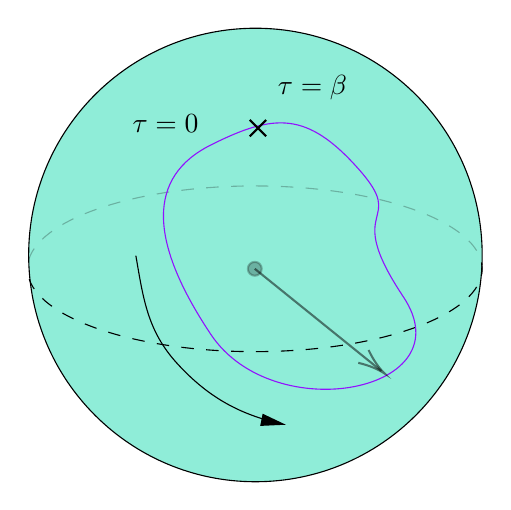
\begin{tikzpicture}[x=0.75pt,y=0.75pt,yscale=-1,xscale=1]
%uncomment if require: \path (0,300); %set diagram left start at 0, and has height of 300

%Shape: Circle [id:dp4271001416525375] 
\draw  [fill={rgb, 255:red, 80; green, 227; blue, 194 }  ,fill opacity=0.64 ] (100.21,156.46) .. controls (100.21,96.12) and (149.12,47.21) .. (209.46,47.21) .. controls (269.79,47.21) and (318.71,96.12) .. (318.71,156.46) .. controls (318.71,216.79) and (269.79,265.71) .. (209.46,265.71) .. controls (149.12,265.71) and (100.21,216.79) .. (100.21,156.46) -- cycle ;
%Shape: Arc [id:dp5416427461491542] 
\draw  [draw opacity=0][dash pattern={on 4.5pt off 4.5pt}] (318.45,160.4) .. controls (318.62,161.29) and (318.7,162.19) .. (318.7,163.09) .. controls (318.7,185.14) and (269.66,203.02) .. (209.16,203.03) .. controls (153.32,203.04) and (107.23,187.82) .. (100.46,168.14) -- (209.15,163.11) -- cycle ; \draw  [dash pattern={on 4.5pt off 4.5pt}] (318.45,160.4) .. controls (318.62,161.29) and (318.7,162.19) .. (318.7,163.09) .. controls (318.7,185.14) and (269.66,203.02) .. (209.16,203.03) .. controls (153.32,203.04) and (107.23,187.82) .. (100.46,168.14) ;
%Shape: Arc [id:dp27514417350783926] 
\draw  [draw opacity=0][dash pattern={on 4.5pt off 4.5pt}] (318.45,165.82) .. controls (318.62,164.93) and (318.7,164.03) .. (318.7,163.13) .. controls (318.7,141.08) and (269.66,123.2) .. (209.16,123.19) .. controls (153.32,123.18) and (107.23,138.4) .. (100.46,158.08) -- (209.15,163.11) -- cycle ; \draw  [color={rgb, 255:red, 0; green, 0; blue, 0 }  ,draw opacity=0.25 ][dash pattern={on 4.5pt off 4.5pt}] (318.45,165.82) .. controls (318.62,164.93) and (318.7,164.03) .. (318.7,163.13) .. controls (318.7,141.08) and (269.66,123.2) .. (209.16,123.19) .. controls (153.32,123.18) and (107.23,138.4) .. (100.46,158.08) ;
%Shape: Polygon Curved [id:ds05822553982795253] 
\draw  [color={rgb, 255:red, 144; green, 19; blue, 254 }  ,draw opacity=1 ] (187.96,103.47) .. controls (218.36,88.26) and (234.23,87.07) .. (258.97,114.83) .. controls (283.71,142.58) and (250.3,130.97) .. (280.71,176.58) .. controls (311.11,222.2) and (218.36,240.31) .. (187.96,194.69) .. controls (157.55,149.08) and (157.55,118.67) .. (187.96,103.47) -- cycle ;
%Straight Lines [id:da6134231895751854] 
\draw [color={rgb, 255:red, 0; green, 0; blue, 0 }  ,draw opacity=1 ]   (210.68,95.34) ;
\draw [shift={(210.68,95.34)}, rotate = 45] [color={rgb, 255:red, 0; green, 0; blue, 0 }  ,draw opacity=1 ][line width=0.75]    (-5.59,0) -- (5.59,0)(0,5.59) -- (0,-5.59)   ;
%Straight Lines [id:da9066706253629926] 
\draw [color={rgb, 255:red, 0; green, 0; blue, 0 }  ,draw opacity=0.5 ][line width=0.75]    (270.15,212.33) -- (209.15,163.11) ;
\draw [shift={(271.71,213.58)}, rotate = 218.9] [color={rgb, 255:red, 0; green, 0; blue, 0 }  ,draw opacity=0.5 ][line width=0.75]    (13.12,-3.95) .. controls (8.34,-1.68) and (3.97,-0.36) .. (0,0) .. controls (3.97,0.36) and (8.34,1.68) .. (13.12,3.95)   ;
%Straight Lines [id:da5443690821222467] 
\draw    (100,149.66) ;
%Straight Lines [id:da23851388151552166] 
\draw [color={rgb, 255:red, 0; green, 0; blue, 0 }  ,draw opacity=0.25 ]   (209.15,163.11) ;
\draw [shift={(209.15,163.11)}, rotate = 0] [color={rgb, 255:red, 0; green, 0; blue, 0 }  ,draw opacity=0.25 ][fill={rgb, 255:red, 0; green, 0; blue, 0 }  ,fill opacity=0.25 ][line width=0.75]      (0, 0) circle [x radius= 3.35, y radius= 3.35]   ;
%Curve Lines [id:da94729558266777] 
\draw    (151.85,156.78) .. controls (155.41,177.15) and (157.29,192.83) .. (171.61,208.56) .. controls (185.57,223.89) and (200.71,233.21) .. (222.42,237.89) ;
\draw [shift={(224.11,238.24)}, rotate = 191.4] [fill={rgb, 255:red, 0; green, 0; blue, 0 }  ][line width=0.08]  [draw opacity=0] (12,-3) -- (0,0) -- (12,3) -- cycle    ;

% Text Node
\draw (149,87.4) node [anchor=north west][inner sep=0.75pt]    {$\tau =0$};
% Text Node
\draw (219,68.4) node [anchor=north west][inner sep=0.75pt]    {$\tau =\beta $};


\end{tikzpicture}

    }
    \subfigure[路径积分中的$(1 - \cos \theta) \partial_\tau \phi$微元]{
        

\tikzset{every picture/.style={line width=0.75pt}} %set default line width to 0.75pt        

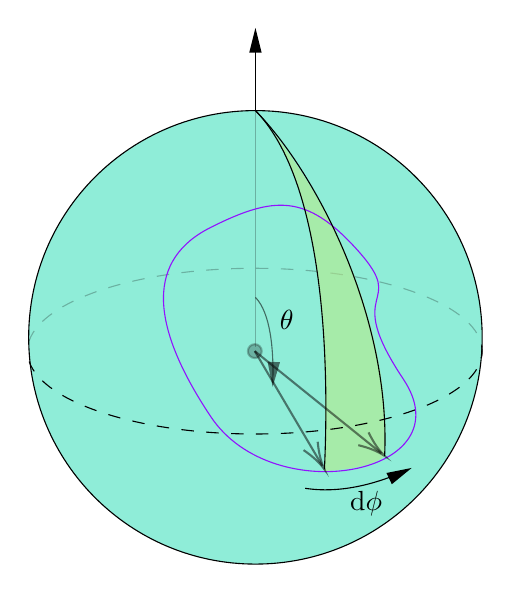
\begin{tikzpicture}[x=0.75pt,y=0.75pt,yscale=-1,xscale=1]
%uncomment if require: \path (0,300); %set diagram left start at 0, and has height of 300

%Shape: Circle [id:dp13786767435744185] 
\draw  [fill={rgb, 255:red, 80; green, 227; blue, 194 }  ,fill opacity=0.64 ] (337.21,163.46) .. controls (337.21,103.12) and (386.12,54.21) .. (446.46,54.21) .. controls (506.79,54.21) and (555.71,103.12) .. (555.71,163.46) .. controls (555.71,223.79) and (506.79,272.71) .. (446.46,272.71) .. controls (386.12,272.71) and (337.21,223.79) .. (337.21,163.46) -- cycle ;
%Shape: Arc [id:dp9522431051366946] 
\draw  [draw opacity=0][dash pattern={on 4.5pt off 4.5pt}] (555.45,172.82) .. controls (555.62,171.93) and (555.7,171.03) .. (555.7,170.13) .. controls (555.7,148.08) and (506.66,130.2) .. (446.16,130.19) .. controls (390.32,130.18) and (344.23,145.4) .. (337.46,165.08) -- (446.15,170.11) -- cycle ; \draw  [color={rgb, 255:red, 0; green, 0; blue, 0 }  ,draw opacity=0.25 ][dash pattern={on 4.5pt off 4.5pt}] (555.45,172.82) .. controls (555.62,171.93) and (555.7,171.03) .. (555.7,170.13) .. controls (555.7,148.08) and (506.66,130.2) .. (446.16,130.19) .. controls (390.32,130.18) and (344.23,145.4) .. (337.46,165.08) ;
%Shape: Polygon Curved [id:ds20966219878034242] 
\draw  [draw opacity=0][fill={rgb, 255:red, 184; green, 233; blue, 134 }  ,fill opacity=0.57 ] (446.46,54.21) .. controls (499.46,116.46) and (511.46,182.1) .. (508.71,220.58) .. controls (504.36,224.5) and (495.56,226.7) .. (479.76,227.9) .. controls (479.96,197.7) and (485.06,94.06) .. (446.46,54.21) -- cycle ;
%Straight Lines [id:da040656680856383076] 
\draw    (446.46,16.32) -- (446.46,54.21) ;
\draw [shift={(446.46,14.32)}, rotate = 90] [fill={rgb, 255:red, 0; green, 0; blue, 0 }  ][line width=0.08]  [draw opacity=0] (12,-3) -- (0,0) -- (12,3) -- cycle    ;
%Straight Lines [id:da786719038701464] 
\draw [color={rgb, 255:red, 0; green, 0; blue, 0 }  ,draw opacity=0.25 ]   (446.46,54.21) -- (446.46,168.23) ;
%Shape: Arc [id:dp9443167576463041] 
\draw  [draw opacity=0][dash pattern={on 4.5pt off 4.5pt}] (555.45,167.4) .. controls (555.62,168.29) and (555.7,169.19) .. (555.7,170.09) .. controls (555.7,192.14) and (506.66,210.02) .. (446.16,210.03) .. controls (390.32,210.04) and (344.23,194.82) .. (337.46,175.14) -- (446.15,170.11) -- cycle ; \draw  [dash pattern={on 4.5pt off 4.5pt}] (555.45,167.4) .. controls (555.62,168.29) and (555.7,169.19) .. (555.7,170.09) .. controls (555.7,192.14) and (506.66,210.02) .. (446.16,210.03) .. controls (390.32,210.04) and (344.23,194.82) .. (337.46,175.14) ;
%Shape: Polygon Curved [id:ds8135273243457903] 
\draw  [color={rgb, 255:red, 144; green, 19; blue, 254 }  ,draw opacity=1 ] (424.96,110.47) .. controls (455.36,95.26) and (471.23,94.07) .. (495.97,121.83) .. controls (520.71,149.58) and (487.3,137.97) .. (517.71,183.58) .. controls (548.11,229.2) and (455.36,247.31) .. (424.96,201.69) .. controls (394.55,156.08) and (394.55,125.67) .. (424.96,110.47) -- cycle ;
%Straight Lines [id:da0919823888859701] 
\draw [color={rgb, 255:red, 0; green, 0; blue, 0 }  ,draw opacity=0.5 ][line width=0.75]    (507.15,219.33) -- (446.15,170.11) ;
\draw [shift={(508.71,220.58)}, rotate = 218.9] [color={rgb, 255:red, 0; green, 0; blue, 0 }  ,draw opacity=0.5 ][line width=0.75]    (13.12,-3.95) .. controls (8.34,-1.68) and (3.97,-0.36) .. (0,0) .. controls (3.97,0.36) and (8.34,1.68) .. (13.12,3.95)   ;
%Straight Lines [id:da7641038914794658] 
\draw    (337,156.66) ;
%Straight Lines [id:da8631491702531824] 
\draw [color={rgb, 255:red, 0; green, 0; blue, 0 }  ,draw opacity=0.25 ]   (446.15,170.11) ;
\draw [shift={(446.15,170.11)}, rotate = 0] [color={rgb, 255:red, 0; green, 0; blue, 0 }  ,draw opacity=0.25 ][fill={rgb, 255:red, 0; green, 0; blue, 0 }  ,fill opacity=0.25 ][line width=0.75]      (0, 0) circle [x radius= 3.35, y radius= 3.35]   ;
%Straight Lines [id:da12016344147570801] 
\draw [color={rgb, 255:red, 0; green, 0; blue, 0 }  ,draw opacity=0.5 ][line width=0.75]    (478.69,225.36) -- (446.15,170.11) ;
\draw [shift={(479.71,227.09)}, rotate = 239.51] [color={rgb, 255:red, 0; green, 0; blue, 0 }  ,draw opacity=0.5 ][line width=0.75]    (13.12,-3.95) .. controls (8.34,-1.68) and (3.97,-0.36) .. (0,0) .. controls (3.97,0.36) and (8.34,1.68) .. (13.12,3.95)   ;
%Curve Lines [id:da7960637854392238] 
\draw    (470.4,236.19) .. controls (490.04,239.21) and (508.96,232.26) .. (520.04,227.17) ;
\draw [shift={(521.73,226.38)}, rotate = 514.62] [fill={rgb, 255:red, 0; green, 0; blue, 0 }  ][line width=0.08]  [draw opacity=0] (12,-3) -- (0,0) -- (12,3) -- cycle    ;
%Curve Lines [id:da46076484070564927] 
\draw    (446.46,54.21) .. controls (476.71,85.2) and (482.71,161.2) .. (479.71,227.09) ;
%Curve Lines [id:da07397623956465105] 
\draw    (446.46,54.21) .. controls (476.71,85.2) and (511.71,154.69) .. (508.71,220.58) ;
%Curve Lines [id:da7251628481913182] 
\draw [color={rgb, 255:red, 0; green, 0; blue, 0 }  ,draw opacity=0.54 ]   (446.46,144.2) .. controls (453.7,151.61) and (455.36,169.37) .. (454.82,185.31) ;
\draw [shift={(454.75,187.3)}, rotate = 272.61] [fill={rgb, 255:red, 0; green, 0; blue, 0 }  ,fill opacity=0.54 ][line width=0.08]  [draw opacity=0] (12,-3) -- (0,0) -- (12,3) -- cycle    ;

% Text Node
\draw (457,149.4) node [anchor=north west][inner sep=0.75pt]    {$\theta $};
% Text Node
\draw (499.79,236.4) node [anchor=north] [inner sep=0.75pt]    {$\mathrm{d} \phi $};


\end{tikzpicture}

    }
    \caption{单自旋的Berry相位图示}
\end{figure}

\section{一维反铁磁海森堡自旋链}

\subsection{低能有效理论和拓扑相}

考虑一维反铁磁海森堡自旋链
\begin{equation}
    H = J \sum_{i} \vb*{S}_i \cdot \vb*{S}_{i+1}, \quad J > 0,
\end{equation}
其自旋路径积分表述为(下面注意区分作用量$S$和自旋长度$S$)
\begin{equation}
    Z = \int \prod_i \fd{\vb*{n}_i} \ee^{-S[\{\vb*{n}_i\}]} , \quad S[\{\vb*{n}_i\}] = \int \dd{\tau} \sum_i ( \ii S (1 - \cos \theta_i) \partial_\tau \phi_i + J S^2 \cos \vartheta_{i, i+1} ),
\end{equation}
其中$\vartheta_{ij}$表示$\vb*{n}_i$和$\vb*{n}_j$之间的夹角。

